\documentclass{endm}
\usepackage{endmmacro}
\usepackage{graphicx}


\usepackage{amssymb,amsmath,latexsym}
\usepackage[varg]{pxfonts}
%%%%%% ENTER ADDITIONAL PACKAGES
%\usepackage{graphics}
\usepackage{pst-all}
\usepackage{graphicx}
\usepackage{amsmath,amsfonts}
\usepackage{amssymb} % ADDED
\usepackage{times}
\usepackage{latexsym}
\usepackage{fancybox}
\usepackage{algorithm}
%\usepackage{algorithmic}
\usepackage{algorithmicx}
\usepackage{algpseudocode}
\usepackage{setspace}
\usepackage{courier}
\usepackage{verbatim}
\usepackage{hhline}
\usepackage{etex}
\usepackage{graphicx}
\usepackage{tikz}
\usetikzlibrary{calc,arrows,automata}
\usetikzlibrary{matrix,positioning,arrows,decorations.pathmorphing,shapes}
\usetikzlibrary{shapes,snakes}
\usepackage{graphicx}
%---------------
\usepackage{subfigure}
\usepackage{mathtools}
\usepackage{booktabs}
\usepackage{hyperref}

\tolerance=1
\emergencystretch=\maxdimen
\hyphenpenalty=10000
\hbadness=10000


\floatname{algorithm}{Algorithm}


\def\lastname{Please list your Lastname here}

\begin{document}


\begin{frontmatter}

\title{Métodos Numéricos 2019 - Obligatorio 1}

\author{Bruno Figares (4391788-8),}
\author{Adrián Gioda (4954044-5),}
\author{Daniel Martinez (4462694-5),}
\author{Adriana Soucoff (3190794-8)}

\address{Instituto de Matem\'atica y Estad\'istica\\ Facultad de Ingenier\'ia. Universidad de la Rep\'ublica\\ Montevideo, Uruguay}

\end{frontmatter}


\section{Ejercicio 1}
\subsection{Representación de $f$ en $\mathbb{R}^2$}
%TODO: fix image positioning
\begin{figure}[htbp]
  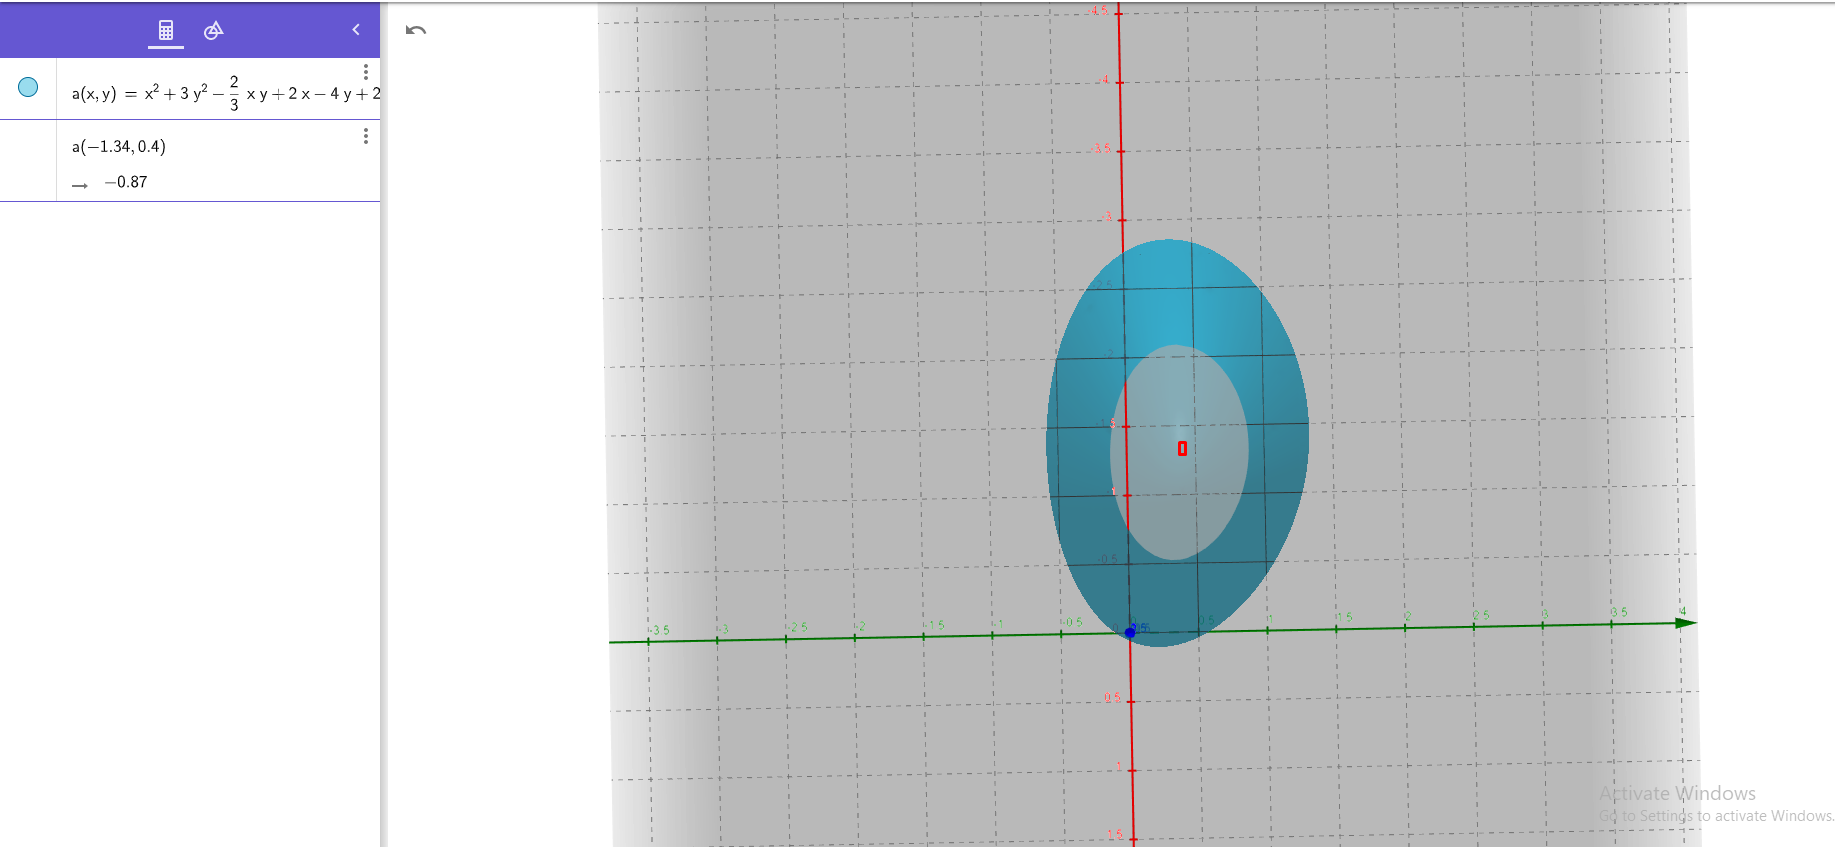
\includegraphics[width=\linewidth]{ej_1_1_1.png}
  \caption{isocurvas de $f(x,y)$}
  \label{fig:1.1.1}
\end{figure}
\begin{figure}[htbp]
  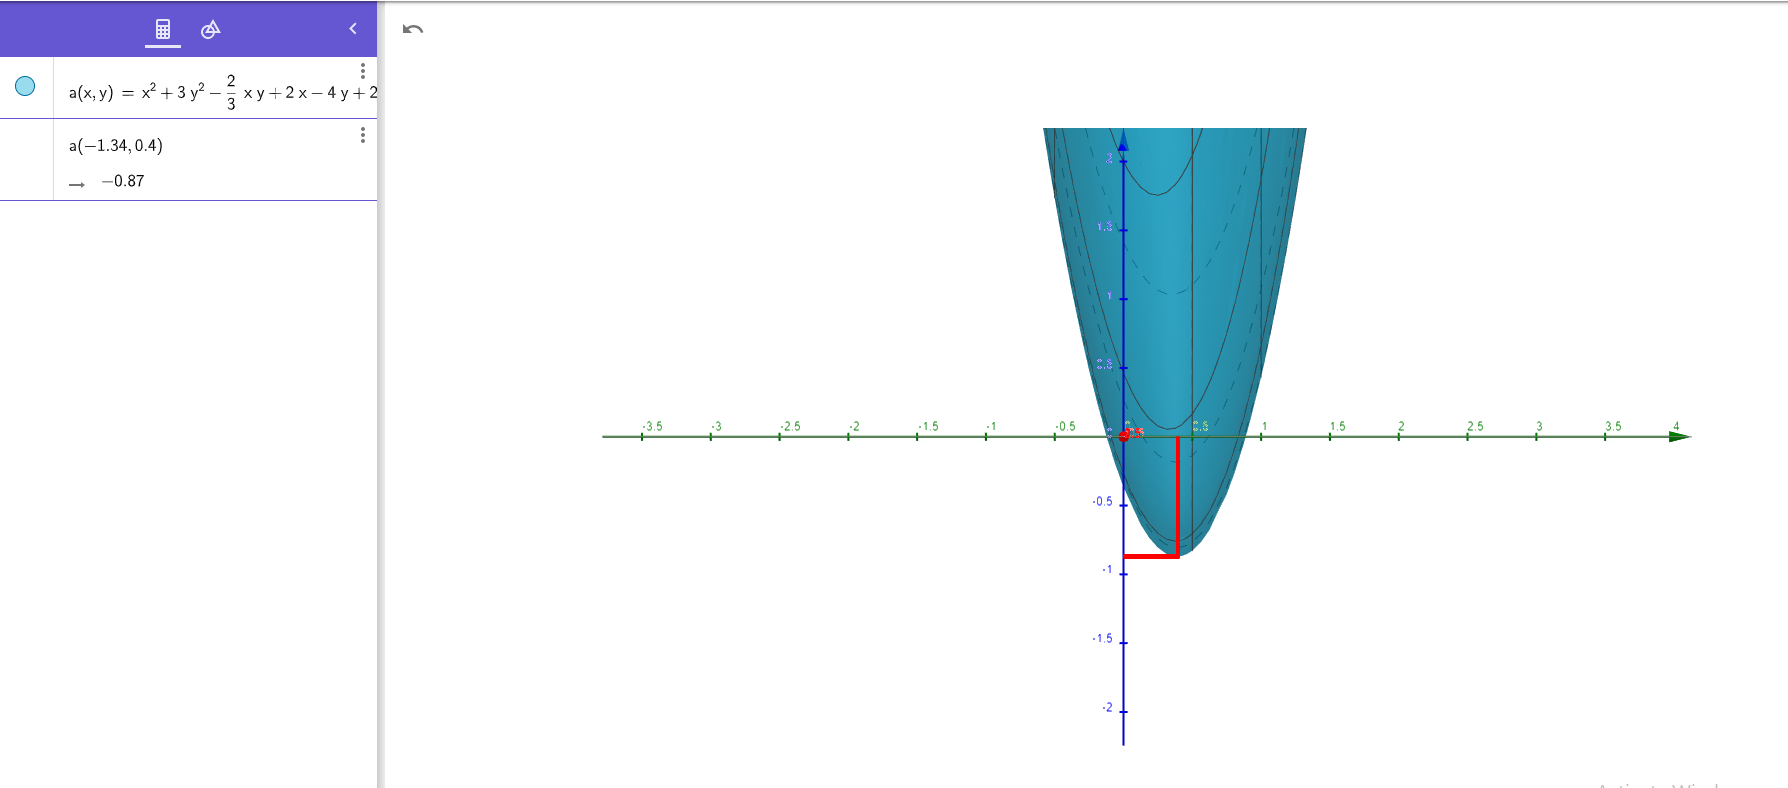
\includegraphics[width=\linewidth]{ej_1_1_2.png}
  \caption{corte transversal de $f(x,y)$}
  \label{fig:1.1.2}
\end{figure}
Se adjuntan dos imágenes  \ref{fig:1.1.1} y \ref{fig:1.1.2}  donde se puede ver la función $f(x,y)$. Su forma parece ser convexa con un mínimo global cerca de cero.
\subsection{Hallar $Q$ y $b$}
$Q \in \mathbb{R}^{2\times2}$ y $b \in \mathbb{R}^{2\times1}$ tienen la siguiente forma

\begin{equation}
    Q = \begin{pmatrix} q_{11} & q_{12} \\ q_{21} & q_{22} \end{pmatrix}
\end{equation}

\begin{equation}
    b = \begin{pmatrix} b_1 \\ b_2 \end{pmatrix}
\end{equation}
Sea

\begin{multline} 
   \\ f(z) = (z^{T}Qz - 2b^{T}z) + 2e^{z_x+z_y} \\
    z = (z_x,z_y)^T \in \mathbb{R}^{2\times1}.\\
\end{multline}
Desarrollando
\begin{equation}
    f(z) = q_{11}z_x^2 + q_{22}z_y^2 + (q_{12} + q_{21})z_x z_y - 2b_1 z_x - 2b_2z_y + 2e^{z_x+z_y}
\end{equation}
Tenemos el siguiente sistema
\begin{equation}
\begin{cases}
q_{11} = 1 \\
q_{12} + q_{21} = -\frac{2}{3} \\
q_{22} = 3 \\
b_1 = -1 \\
b_2 = 2
\end{cases}
\end{equation}

Resolviendolo se tiene que
$Q =  \begin{pmatrix} 1 & -\frac{1}{3} \\ -\frac{1}{3} & 3\end{pmatrix} $
y
$b = \begin{pmatrix} -1\\ 2 \end{pmatrix}$
\subsection{$F(z) = (Qz -b)+ e^{x+y}$}

\subsection{}
\subsection{}
 


Let us develop an ILP for the problem under study. The key idea is to consider connectivity requirement $r_q=2$ for every pair of terminals $q$ from the backbone, while $r_q=1$ otherwise.
Let $Q=\{q=(i,j),\forall i\neq j, i,j \in T\subseteq V\}$. Consider the following set of binary variables:
\begin{itemize}
\item  $z_{ij}=1$ iff $(i,j)\in E$ is in the backbone;
\item $y_{ij}=1$ iff $(i,j)\in E$ is in the access network;
\item $x_{ij}^{q}$ is the $i-j$ flow for every pair of terminals $q$;
\item $p_{i}=1$ iff the $i$ is included in the access network.
\end{itemize}

An ILP formulation for the 2NCSP-SN can be expressed as follows:

%TODO PASAR A FORMATO ALIGN; ACOMODAR EN UNA SOLA RESTRICCION LA QUE APARECE CON LLAVES
\setcounter{equation}{0}
\begin{align}
\small
\mbox{min}_{H \subseteq G} &c(H)= \sum _{ij\in E} c_{ij}.z_{ij}+ \sum _{s\in S} a_{s}.p_{s}+ \sum _{ij\in E} d_{ij}.y_{ij}\label{ecu0} \\
\mbox{s.t.} &\sum _{j:(j,i)\in E} x_{ji}^{q}-\sum _{j:(i,j)\in Ed^{q}} x_{ij}^{q} =  I(i).r_{i}\: \forall i \in V,\:\forall q=(q_{o},q_{d})\in Q \label{ecu1}\\
& I(i)=1 \:\forall i \in V \backslash \{q_{o}\},\:I(q_{o})=-1 \label{ecu2}\\
& r_{i}= 0 \:\forall i \in V \backslash \{q_{o},q_{d}\} \label{ecu3}\\
& \max(1,p_{q_{o}}+p_{q_{d}}) \leq r_{i}\leq 1+ \min(p_{q_{o}},p_{q_{d}}),\:\forall  i \in \{q_{o},q_{d}\},\:\forall q\in Q\label{ecu4}\\
& x_{ij}^{q}+x_{ji}^{q} \leq z_{ij}+y_{ij},  \:\forall ij\in E,\:\forall q \in Q \label{ecu5}\\
& \sum_{j \in \delta (i)} y_{ij} \leq  1+ M p_{i}, \:\forall  i\in T \label{ecu6}\\
&\sum _{j\in \delta (i)} (z_{ij}+y_{ij}) \leq  M p_{i}, \:\forall  i\in S \label{ecu7}\\
& y_{ij} \leq 2-p_{i}-p_{j}, \: \forall ij\in E, i,j \in V\label{ecu8}\\
& z_{ij} \leq \min(p_{i},p_{j}), \: \forall ij\in E, i,j \in V\label{ecu9}\\
& z_{ij}+y_{ij} \leq 1 \: \forall ij\in E, i,j \label{ecu10}\\
& 2p_{i} \leq \sum_{j\in \delta (i)}z_{ij}\leq Mp_{i}, \: \forall i \in V\label{ecu11}
\end{align}

Where $\delta (i)$ is neighbor-set for node $i$, and $M$ is an arbitrarily large integer.
The objective function~\eqref{ecu0} is the contribution of internal/external connections and Steiner nodes. Constraints~\eqref{ecu1}-\eqref{ecu4} ensure connectivity using Kirchhoff equations.
%When the pair of terminals $q$ belongs to the backbone, $r_{i}=2, i\in \{q_{o},q_{d}\}$;
%otherwise $r_{i}=1$.
Constraints~\eqref{ecu5}~and~\eqref{ecu6} force one-way flow.
By Constraint~\eqref{ecu7}, optional Steiner nodes belong to the backbone, if needed.
The definitions of binary variables $y_{ij}$ and $z_{ij}$ are captured by Constraints~\eqref{ecu8}
and~\eqref{ecu9}. Constraints~\eqref{ecu10} state that either $y_{ij}$  or $z_{ij}$ can be set to $1$, but not both. 
Constraints~\eqref{ecu11} state that a terminal from the backbone could have multilinks, but nodes from the access network have one link.

\section{Methodology}\label{AA}
From now on, we assume that the internal/external costs are positive and internal costs satisfy the triangle inequality. Without loss of generality, a complete graph $G=(V,E)$ is considered. Let $\alpha_{e}=\frac{c_e}{d_e}, \forall e \in E$ be the primary/secondary cost ratio for each arc.
In this section we build an approximation algorithm for the the 2NCSP-SN of factor $4\alpha$,
being $\alpha$:
\begin{equation}
\alpha = \max_{e\in E} \left\{\alpha_{e} \right\}
\end{equation}

Recall that Christofides's algorithm is a 3/2-factor for the metric TSP.
The key concept of our approximation algorithm is Christofides in order to span the terminal-set
with an elementary cycle. Greedy augmentations of the solution including Steiner nodes also takes place, whenever the cost is reduced.

In Line~1, $Christofides$ is called in order to build an elementary cycle $\mathcal{C}$
that spans the terminal-set $T$. The corresponding solution is updated in Lines 2-3,
where the backbone is $\mathcal{C}$ and the access network is empty yet.
In the while-loop (Lines 4-11),
Steiner nodes are greedily included in the backbone, whenever the cost is reduced (Line 5).
If this happens, some terminal node $v$ is included in the access network, and the
evidence $s \in S$ is added to the backbone (Lines 6-7). Observe that candidate terminals
$t \in T$ are iteratively checked (Line 9), and the condition $|J|\geq 3$ forces to have
a cycle in the backbone. The corresponding feasible solution $F$ is finally returned (Line 12).

\begin{algorithm}[H]
\small
\centering
\begin{algorithmic}[1]
\Require $G=(T\cup S,E)$,$c(e),d(e) \forall e \in E$,
\State {$\mathcal{C} \leftarrow Christofides(G,c)$ }
\State {$L \leftarrow \emptyset$, $I \leftarrow T$, $E^{\prime} \leftarrow E(\mathcal{C})$, $J \leftarrow T$}
\State {$F \leftarrow (L\cup I,E^{\prime})$}
%\Comment {Introduce Steiner nodes to the Backbone if the cost is reduced:}
\While{$|J| \geq 3$}
    \If {there are  $s \in S$, $(t,v),(v,w)\in F$: $c(t,v)+c(v,w)>d(v,s)+c(t,s)+c(s,w)$}
            \State {$L \leftarrow L\cup \{v\}$, $I \leftarrow I \cup \{s\}\:  \backslash\: \{v\}$, $J \leftarrow J \backslash \{t,v\}$ }
            \State {$E^{\prime} \leftarrow E^{\prime} \cup \{(t,s),(s,v),(s,w)\}\:\backslash\: \{(t,v),(v,w)\} $ }
         \Else
           \State {$J \leftarrow J \:\backslash\: \{t\}$}
    \EndIf
\EndWhile \\
\Return $F=(I\cup L,E^{\prime})$
\end{algorithmic}
\end{algorithm}

\clearpage

\begin{lem}\label{lema}
If $L(F) \neq \emptyset$ then $\alpha>1/2$
\end{lem}
\begin{proof}
By the triangle inequality, $c_{(t,v)}\leq c_{(t,s)}+c_{(s,v)}$ and
$c_{(v,w)}\leq c_{(v,s)}+c_{(s,w)}$, so
$c_{(t,v)}+c_{(v,w)} \leq c_{(t,s)}+2.c_{(s,v)}+ c_{(s,w)}$. If $L \neq \emptyset$, there exists $v \in L$, $s \in S \cap I, t,w \in I$ such that
$c_{(t,v)}+c_{(v,w)}>d_{(v,s)}+c_{(t,s)}+c_{(s,w)}$,\\ %\, d_{(v,s)}= c_{(v,s)}/\alpha$.\\
Therefore $d_{(v,s)} = c_{(v,s)}/\alpha_{v,s }< 2.c_{(s,v)}$, so there exists $e=(v,s)$ such that $\alpha_{e} > 1/2$, that is $\alpha > 1/2$ with $\alpha = \max_{e\in E} \left\{\alpha_{e} \right\}$.

\end{proof}
%According to Lemma~\ref{lema}, if $\alpha \geq 2$ then $F$ is an elementary cycle without Steiner nodes.
\begin{thm}
$c(F) \leq \max\{2,4 \alpha\}\times  OPT$.
\end{thm}

\begin{proof}
Let $G^*=(S^* \cup T,E^*)$ be the optimal solution, $H$ the cheapest Hamilton tour spanning $T$  and $H^S$ the cheapest Hamilton tour spanning $T\cup S^*$.
Analogously, let us denote $TNC$ ($TEC$) to the optimal 2-node (resp. 2-edge) connected spanning subgraph for $T\cup S^{*}$. Recall that $F$ is the output and $\mathcal{C}$ the cycle obtained
using Christofides algorithm. Combining Monma and Christofides theorems:
\begin{equation}\label{1}
c(G^{*}) \leq c(F) \leq c(\mathcal{C})\leq \frac{3}{2}c(H)
                   \leq \left(\frac{3}{2}\right) \left(\frac{4}{3}\right) c(TNC) = 2 c(TNC)
\end{equation}
Let $G^{*}=B \cup L$, being $B$ its backbone. Consider an augmentation $F^{\prime}$ for $G^{*}$, doubling edges from $L$
with cost $c_{r,j}=\alpha_{r,j} d_{r,j}$ and adding them. $F^{\prime}$ is 2-edge connected and
\begin{equation}\label{2}
c(F^{\prime}) = c(B)+2\sum_{r\in L}c_{r,j} \leq c(B)+2\alpha \sum_{r\in L}d_{r,j} =2 \alpha c(G^{*})+(1- 2 \alpha)c(B),
\end{equation}
\indent If $1-2 \alpha > 0$, $c(F^{\prime}) \leq 2 \alpha c(G^{*})+ 2(1-2 \alpha )c(G^{*})\leq 2 c(G^{*})$.
In this case a factor 2 is provided, and by Lemma~\ref{lema} $F$ consists of an elementary cycle.

\indent Otherwise, combining~\eqref{1}~and~\eqref{2} we have that:
\begin{align*}
  c(G^{*}) & \leq c(F) \leq 2 c(TNC) = 2 c(TEC) \leq 2 c(F^{\prime}) \\
           & \leq 4 \alpha c(G^{*})+ 2(1-2 \alpha)c(B)\\
           &\leq 4\alpha c(G^{*}).
\end{align*}
\end{proof}

\clearpage
\section{Experimental Analysis}\label{Comparison}
In order to highlight the effectiveness of our approximation algorithm, a sensibility
analysis with respect to the ratio $\alpha$ is carried out. We consider a single
instance from TSPLIB named berlin52.tsp. This is the case of a real-life network
with Euclidean costs. In order to find the globally optimum solution, an
induced subgraph with 22 nodes is considered (with 10  terminal-nodes and 12 Steiner nodes).
The ILP has been executed in CPLEX 12.6.3 MIP solver using an Intel i7 processor, 2.30 GHz, 8GB RAM.
Table~\ref{Table:resul1} illustrates the performance $c(F)/OPT$ as a function
of $\alpha$. The cycle $\mathcal{C}$ obtained using Christofides algorithm is
$c(\mathcal{C})=3164.8$, while the cheapest Hamiltonian tour $H$ spanning the terminal-set
has a cost $c(H)=2826.5$. Naturally, since $F$ considers greedy augmentations of
$\mathcal{C}$, we get that $c(F)\leq c(\mathcal{C})$ in all cases.

\begin{table}[H]
\caption{Sensibility Analysis as a function of $\alpha$ \label{Table:resul1}}
\centering
\begin{tabular}{l|r|r|r|r|r}
\toprule
& $\alpha$  & $OPT$ & $c(F)$ & $c(F)/OPT$\\
\midrule
&   10 & 485.78 & 3117.3  & 6.42  \\
&   4 & 1110.48 & 3164.8  & 2.85  \\
&   2 & 2115.02 & 3164.8  & 1.50   \\
&   4/3 & 2611.45 & 3164.8  & 1.21 \\
&   1 & 2786.80  & 3164.8  & 1.14   \\
&   4/5 & 2811.63  & 3164.8  & 1.13 \\
&   2/3 & 2822.88  & 3164.8   & 1.12 \\
&   4/7 & 2825.60  & 3164.8  & 1.12  \\
\bottomrule
\end{tabular}
\end{table}
.

\clearpage
\end{document}\grid
